%==============================================================================
%  Certified Optimal Defence in a Path-Contest Network Security Game
%  ICORES submission version.
%
%  Compile:  pdflatex icores.tex   (run twice for cross-references)
%
%  TEMPLATE NOTE.  This file compiles standalone with a stock LaTeX
%  installation, and its layout follows the SCITEPRESS conventions used by
%  INSTICC proceedings (A4, twoside, single column, author-year citations in
%  apalike style, numbered sections, an ACKNOWLEDGEMENTS section before the
%  references).  To move it onto the official class once the target template
%  is confirmed, replace the \documentclass line and the geometry/natbib
%  lines below with
%
%      \documentclass[a4paper,twoside]{article}
%      \usepackage{apalike}
%      \usepackage{SCITEPRESS}
%
%  and copy apalike.bst, apalike.sty, article.cls and SCITEPRESS.sty into
%  this directory.  Nothing in the body needs to change.
%==============================================================================

\documentclass[10pt,a4paper,twoside]{article}

\usepackage[T1]{fontenc}
\usepackage[utf8]{inputenc}
\usepackage{times}
\usepackage{amsmath,amssymb,amsthm}
\usepackage{booktabs}
\usepackage{graphicx}
\usepackage[margin=2.5cm]{geometry}
\usepackage[authoryear,round]{natbib}
\usepackage{enumitem}
\usepackage{caption}

\bibpunct{(}{)}{;}{a}{,}{,}

\theoremstyle{plain}
\newtheorem{theorem}{Theorem}
\newtheorem{proposition}[theorem]{Proposition}
\newtheorem{lemma}[theorem]{Lemma}
\newtheorem{corollary}[theorem]{Corollary}
\theoremstyle{definition}
\newtheorem{remark}[theorem]{Remark}

\newcommand{\XA}{\bar{x}_A}
\newcommand{\XB}{\bar{x}_B}
\newcommand{\Path}{\mathcal{P}}

\captionsetup{font=small,labelfont=bf}
\setlength{\parskip}{0pt}

\begin{document}

\title{\bf Certified Optimal Defence in a Path-Contest\\ Network Security Game}

% TODO(author): author names, affiliations and e-mail addresses.
\author{}
\date{}
\maketitle

%==============================================================================
\begin{abstract}
\noindent
A defender spreads a fixed budget over the nodes of a directed graph. An
evader observes the allocation, chooses a source--destination route, and
spreads its own fixed budget over the nodes of that route. Each node is a
ratio-form (Tullock) contest of intensity $m$, and the evader must survive
every node on its route, so its success probability is a product of per-node
terms. We prove that in logarithmic coordinates the defender's objective is
convex for $m\le1$, which makes the Stackelberg value computable to a
certified global optimum rather than to a stationary point, and we exhibit a
graph on which convexity fails at $m=2$. We also prove that the optimal
allocation is unique when the game is non-degenerate; the argument is a
covering argument, since the objective is not strictly convex. Two
algorithmic ingredients follow from the structure: a Lagrangian relaxation
that is additive over nodes reduces the evader's route choice to a single
shortest-path computation with a stopping rule that certifies when no
unexamined route can be better, and the defender's allocation is obtained by
cutting planes with a stabilised master, giving two-sided bounds. The solver
reproduces four independently derived closed-form families to
$5.75\times10^{-12}$ and passes 80 automated checks. On layered graphs with
up to $1.68\times10^{7}$ routes the oracle examines two routes per best
response, and the optimality certificate closes on all 13 instances tested.
Even budget allocation is optimal on the symmetric families we analyse but
raises the evader's success probability by $211\%$ on average over 20
irregular graphs.
\end{abstract}

\noindent\textbf{KEYWORDS:} network interdiction; Tullock contest;
Stackelberg games; convex optimisation; cutting-plane methods.

\medskip

%==============================================================================
\section{INTRODUCTION}
\label{sec:intro}

A network defender rarely chooses where an intrusion happens. It chooses only
how to spread a limited protective budget, and must commit before the
intrusion occurs. The intruder usually sees the defence, since guards,
checkpoints and sensors are visible, and routes around the strong points.

We study a direct mathematical form of that situation. A defender $A$ spreads
a budget $\XA$ over the nodes of a directed graph. An evader $B$ observes the
allocation, picks a route from a source $S$ to a destination $D$, and spreads
a budget $\XB$ over the nodes on that route. At a node with defence $x_i$ and
attack $y_i$ the evader passes with probability
\begin{equation}
  p_i \;=\; \frac{y_i^{\,m}}{x_i^{\,m}+y_i^{\,m}},
  \label{eq:csf}
\end{equation}
the ratio-form contest standard in conflict theory
\citep{tullock1980,skaperdas1996}, where $m>0$ controls how strongly the
larger investment is rewarded. The evader must survive every node on its
route, so the quantity of interest is
\begin{equation}
  V^{\star}
  \;=\;
  \min_{x}\;\max_{P}\;\max_{y}\;
  \prod_{i\in P}\frac{y_i^{\,m}}{x_i^{\,m}+y_i^{\,m}}.
  \label{eq:game}
\end{equation}

Three features make \eqref{eq:game} awkward. The evader's route set can be
exponentially large, the defender's allocation ranges over a continuum, and
the objective as written is neither convex nor concave. Earlier work on
related models has used metaheuristics without optimality guarantees
\citep{ramirez2011} or discrete formulations solved as integer programs
\citep{nguyen2023}.

Our first result is that for $m\le1$ the objective of \eqref{eq:game} is
convex once written in logarithmic coordinates (Theorem~\ref{thm:convexity}),
so the problem admits a certified global optimum. The restriction is sharp in
the sense that we exhibit a graph on which convexity fails at $m=2$
(Proposition~\ref{prop:m-gt-1}), so the boundary is a property of the model
and not an artefact of the proof. Convexity alone does not give a unique
minimiser, and $G$ is in fact not strictly convex; we nevertheless prove
uniqueness of the optimal allocation when $V^{\star}<1$, by combining strict
convexity along an active route with a covering argument
(Lemma~\ref{lem:active-cover}, Proposition~\ref{prop:uniqueness}).

On the algorithmic side, the evader's route choice is a maximum-reliability
path problem. \citet{nguyen2023} prove NP-hardness for the analogous problem
in their discrete setting; that result does not establish NP-hardness of the
continuous model of Section~\ref{sec:model}, and we claim no such reduction.
It does motivate a certified route-generation procedure rather than a search
for a polynomial exact oracle. A Lagrangian relaxation of the evader's split
is additive over nodes, which turns the route search into one shortest-path
computation and supplies a rule proving when no unexamined route can be
better (Section~\ref{sec:oracle}). The defender's problem is then solved by
cutting planes with a stabilised master (Section~\ref{sec:cutting}).

Section~\ref{sec:closed-form} derives exact solutions for four graph families
and a worked example, used as ground truth. Section~\ref{sec:results} reports
the computational study.

%==============================================================================
\section{RELATED WORK}
\label{sec:related}

\paragraph{Network interdiction.}
The classical literature places an interdictor who modifies the network
against an evader who routes through what remains
\citep{washburn1995,israeli2002}; see \citet{smith2020} for a survey.
\citet{nguyen2023} study a two-stage game in which an evader crosses a
network and its payoff is a product of per-arc survival probabilities, the
same series-system structure we use. Their defender's choices are discrete
and their second stage is simultaneous, which forces mixed strategies and a
linear program over path distributions. Our defender's choice is a continuous
budget split and play stays sequential, so a pure optimum exists. Two of
their ideas have direct analogues here: constraint generation over paths
corresponds to our cutting planes, and turning a product of survival
probabilities into a shortest-path problem by taking logarithms corresponds
to our Lagrangian oracle.

\paragraph{Contest models of protection.}
\citet{ramirez2011} use a ratio-form contest of the same family as
\eqref{eq:csf} and report, as an empirical finding, that splitting the
defence budget evenly is optimal when every component is equally vulnerable.
Our symmetric-topology results give a theorem-level counterpart within our
model and locate where the finding stops holding: it is exact on the
symmetric families we analyse and degrades quickly once the graph is
irregular (Section~\ref{sec:results-topologies}). Their setup differs from
ours in its treatment of component values and attacker strategies, so we
prove nothing about their model. Their solution method is an evolutionary
algorithm without an optimality guarantee.

\citet{hausken2008} studies attack and defence of series and parallel
reliability systems with contest success functions, documenting how $m>1$
produces increasing returns to out-investing the opponent. That behaviour is
consistent with the loss of convexity we identify in
Proposition~\ref{prop:m-gt-1}, although that work does not establish the same
non-convexity result.

\paragraph{Attack and interception in networks.}
In \citet{bloch2023} an attacker picks a target and a route while each node
privately decides how much to invest. Their game is decentralised: node $i$
maximises a payoff of the form $-\alpha_i(1-x_i)q_ib_i-x_i^2/2$, a private
quadratic cost with no budget linking nodes, whereas our defender solves one
joint allocation problem under $\sum_i x_i=\XA$. The factor $(1-x_i)$ is
linear in the investment rather than a contest against an opposing
investment, and their attacker chooses only a distribution over targets and
routes. Their solution concept is simultaneous Nash equilibrium and their
uniqueness result concerns that equilibrium; neither result implies the
other.

\paragraph{Attack-graph defence.}
The closest structural relative we found is \citet{oruganti2023}, who study
defence of a cyber-physical system modelled as an attack graph. Play is
Stackelberg with the defender first, the defender spreads a single budget
over the nodes of a directed acyclic graph, the attacker chooses a path, and
the payoff along a path is a product of per-node terms, giving an objective
of the same shape as \eqref{eq:game}. The decisive difference is that their
model has no attacker-side investment and therefore no contest at any node:
their per-node compromise probability is $p_i(x_i)=p_i^{0}e^{-\kappa_i x_i}$
and the attacker picks only a route. In our model the second player is also
budget-constrained and invests node by node. That change generates the inner
maximisation over $y$ and its reduction to a scalar root, the Lagrangian
relaxation of that inner problem, and the convexity theorem itself, whose
content is how $g_P$ depends on $x$ after the evader has re-optimised against
it. Their exponential form makes each route objective log-linear in $x$, so
the two convexity analyses are not the same argument.

\citet{iliaev2023} also use a Tullock contest and compare sequential with
simultaneous play, but their targets are independent and there is no routing
problem. \citet{bozbay2018} define a contest success function on a network of
friendly and hostile relationships, a different use of the word network.

\paragraph{On novelty.}
Our search covered the two papers that motivated the project, targeted
searches on Tullock contests on networks, sequential interdiction with
ratio-form contests, network extensions of the Colonel Blotto game
\citep{kovenock2018}, and the attack-graph defence literature. It is a
keyword search rather than a systematic review. We found no exact match for
the combination used here, namely a single jointly-budgeted defender, a
ratio-form contest at each node, a series-system path payoff, and sequential
play solved to a certified optimum, but absence from a search is evidence
rather than proof.

\paragraph{Algorithms.}
The outer solver is Kelley's cutting-plane method \citep{kelley1960},
stabilised by the boxstep device of \citet{marsten1975}. The gradient comes
from Danskin's theorem \citep{danskin1967} and routes are generated in cost
order by Yen's algorithm \citep{yen1971}.

%==============================================================================
\section{MODEL}
\label{sec:model}

Let $G=(V,E)$ be a directed graph with source $S$ and destination $D$, and
let $\Path$ be the set of simple $S$--$D$ routes. For a route $P$ write
$P^{\circ}$ for its \emph{contested} nodes, by default every node of $P$
except $S$ and $D$. Let $V^{\circ}$ be the set of nodes lying on at least one
route, with $n=|V^{\circ}|$; budget placed elsewhere affects no payoff.

The defender picks $x\ge0$ with $\sum_{i\in V^{\circ}}x_i=\XA$. The evader,
after observing $x$, picks $P$ and a split $y\ge0$ on $P^{\circ}$ with
$\sum_{i\in P^{\circ}}y_i=\XB$. The payoff is
\begin{equation}
  U_B(P,x,y)\;=\;\prod_{i\in P^{\circ}}
  \frac{y_i^{\,m}}{x_i^{\,m}+y_i^{\,m}}.
  \label{eq:payoff}
\end{equation}
Play is sequential, so this is a Stackelberg game and only the value
$V^{\star}$ of \eqref{eq:game} is well defined as a solution concept. A
simultaneous version would in general require mixed strategies over routes,
the setting of \citet{nguyen2023}, and is not treated here.

Two conventions fix the boundary behaviour of \eqref{eq:payoff}. Each is the
only choice under which the value function remains continuous.

\textbf{(C1) Zero defence means free passage.} If $x_i=0$ then
\eqref{eq:csf} gives $p_i=1$ for every $y_i>0$, so the evader spends nothing
at $i$. We set $p_i=1$ when $x_i=0$.

\textbf{(C2) Work in logarithms.} Write
$h(x,y)=\sum_{i\in P^{\circ}}[m\log y_i-\log(x_i^m+y_i^m)]$,
$g_P(x)=\max_y h(x,y)$ for the evader's best split on a fixed route, and
$G(x)=\max_P g_P(x)$, so that $V^{\star}=\exp(\min_x G(x))$. Besides avoiding
underflow on long routes, where raw products reach $10^{-300}$, this is the
coordinate system in which the problem is convex.

\begin{proposition}[The defended set must be a cut]
\label{prop:cut}
If $\{i:x_i>0\}$ does not intersect every $S$--$D$ route, some route is
entirely undefended and the evader succeeds with probability $1$.
\end{proposition}

\noindent This is immediate from (C1). It is the link to the minimum-cut view
of interdiction and it explains an experimental result reported below: a rule
that concentrates budget on a few high-centrality nodes can leave a route
open and so achieve the worst possible outcome.

%==============================================================================
\section{THE EVADER'S PROBLEM}
\label{sec:inner}

Fix a route $P$ and a defence $x$. For $x_i>0$ write
$\varphi_i(y)=m\log y-\log(x_i^m+y^m)$.

\begin{proposition}[Strict concavity]
\label{prop:concave}
For every $m>0$ and every $x_i>0$, $\varphi_i$ is strictly concave on
$(0,\infty)$.
\end{proposition}
\begin{proof}
$\varphi_i'(y)=m x_i^m/[y(x_i^m+y^m)]>0$. The denominator is strictly
increasing in $y$ and the numerator is constant, so $\varphi_i'$ is strictly
decreasing.
\end{proof}

The hypothesis $x_i>0$ is not cosmetic. At $x_i=0$ the numerator vanishes,
$\varphi_i'\equiv0$, and $\varphi_i$ is constant, which is convention (C1):
the node is free and the evader spends nothing there. Strict concavity, and
the uniqueness statements that follow from it, are therefore claims about the
active set $\{i\in P^{\circ}:x_i>0\}$.

On that set the evader's problem has a unique maximiser $y^{\star}(x)$.
Writing $\lambda$ for the budget multiplier and $t=1/\lambda$, stationarity
reads
\begin{equation}
  y_i(x_i^m+y_i^m) \;=\; t\,m\,x_i^m .
  \label{eq:stationarity}
\end{equation}
The left side is strictly increasing in $y_i$, so $y_i(t)$ is unique and
strictly increasing in $t$, hence $\sum_i y_i(t)$ is strictly increasing and
the budget-feasible $t^{\star}$ is the unique root of
$\sum_i y_i(t)=\XB$. The implementation brackets that root and locates it by
safeguarded Newton iterations, falling back on the bracket midpoint whenever
a Newton step would leave the bracket. What is returned is a numerical
solution to a stated tolerance, not a symbolic one, and the accompanying code
reports the root, budget and stationarity residuals.

At $m=1$, \eqref{eq:stationarity} is the quadratic $y^2+x_iy-tx_i=0$ with
cancellation-free positive root
\begin{equation}
  y_i(t)=\frac{2x_it}{x_i+\sqrt{x_i^2+4x_it}},
  \quad
  p_i(t)=\frac{2t}{x_i+2t+\sqrt{x_i^2+4x_it}} .
  \label{eq:m1-closed}
\end{equation}
The textbook form $y=(-x_i+\sqrt{x_i^2+4x_it})/2$ is algebraically identical
but subtracts two nearly equal numbers when $4x_it\ll x_i^2$. That regime
occurs in practice, because the cutting-plane iterates of
Section~\ref{sec:cutting} approach the boundary of the budget simplex.

If every node of a route carries the same defence $x_i=c>0$, then symmetry
and uniqueness give $y_i=\XB/n$ with $n=|P^{\circ}|$, so
\begin{equation}
  U_B = \left(\frac{\XB}{nc+\XB}\right)^{\!n}.
  \label{eq:symmetric}
\end{equation}
The exponent carries much of the behaviour reported later: the evader's
success decays geometrically in route length, so a short route needs more
defence per node than a long one.

\begin{proposition}[Gradient of the inner value]
\label{prop:danskin}
Let $x_i>0$ and let the unique optimal split $y^{\star}$ be strictly positive
on the active set, so that $g_P$ is differentiable at $x$. Then
$\partial g_P/\partial x_i=-mx_i^{m-1}/(x_i^m+(y_i^{\star})^m)$, which at
$m=1$ is $-1/(x_i+y_i^{\star})$.
\end{proposition}

\noindent This is Danskin's theorem \citep{danskin1967}, since $g_P$ is a
maximum over a compact set not depending on $x$ and the maximiser is unique.
The assumptions are stated because they are not automatic: at $x_i=0$ the
function is nonsmooth, the expression above diverges as $x_i\to0^{+}$ when
$m=1$, and no derivative is claimed there. Solving the inner problem once
yields both the value and a gradient at no extra cost, which is what drives
the outer algorithm.

%==============================================================================
\section{CONVEXITY AND UNIQUENESS}
\label{sec:convexity}

\begin{theorem}[Convexity for $m\le1$]
\label{thm:convexity}
For $0<m\le1$, $G$ is convex on the defender's budget simplex.
\end{theorem}
\begin{proof}
Fix $y>0$ and consider one term of $h(x,y)$ as a function of $x_i$, namely
$-\log(x_i^m+y_i^m)$. Write it as $-\log(u+y_i^m)$ with $u=x_i^m$. For
$m\le1$ the map $x_i\mapsto x_i^m$ is concave, and $u\mapsto-\log(u+y_i^m)$
is convex and non-increasing. A convex non-increasing function composed with
a concave function is convex, so each term is convex in $x_i$; the monotonicity
is what licenses the composition. The terms $m\log y_i$ do not involve $x$,
so $h(\cdot,y)$ is convex in $x$ for every fixed feasible $y$.

Then $g_P(x)=\sup_y h(x,y)$ is a supremum of convex functions over a set that
does not depend on $x$, hence convex, and $G=\max_P g_P$ is a maximum of
finitely many convex functions, hence convex. Under (C1) the identity
$-\log(0+y_i^m)+m\log y_i=0$ holds, so $h(\cdot,y)$ extends continuously and
convexity holds up to the boundary of the simplex.
\end{proof}

This makes \eqref{eq:game} a convex program for $m\le1$: every local minimum
is global, and the cutting-plane lower bound of Section~\ref{sec:cutting} is
a valid global under-estimator, so the method can return a certified optimum
whenever the reported gap closes within the requested tolerance. It does not
follow that the minimiser is unique, and indeed $G$ is not strictly convex:
$g_P$ does not depend on the defence variables of nodes off $P$, so two
allocations differing only at such nodes give equality rather than strict
inequality. Strict convexity does hold in a restricted sense.

\begin{proposition}[Strict convexity on the maximising route]
\label{prop:partial-strict}
Let $m=1$, let $x\ne x'$ be two allocations, let $t\in(0,1)$, and let
$P^{\star}$ attain the maximum in $G$ at $z=tx+(1-t)x'$. If $x$ and $x'$
differ in at least one coordinate of $P^{\star\circ}$, and the evader's
optimal split at $z$ puts positive effort on every node of $P^{\star\circ}$,
then $G(z)<t\,G(x)+(1-t)\,G(x')$.
\end{proposition}
\begin{proof}
Let $y^{\star}$ be the evader's optimal split on $P^{\star}$ at $z$, unique
by Proposition~\ref{prop:concave}. Each term $-\log(x_i+y^{\star}_i)$ has
second derivative $1/(x_i+y^{\star}_i)^2>0$ for $x_i\ge0$, so
$h(\cdot,y^{\star})$ restricted to the coordinates of $P^{\star\circ}$ is a
sum of strictly convex functions of separate coordinates. Since $x$ and $x'$
differ in at least one such coordinate,
$h(z,y^{\star})<t\,h(x,y^{\star})+(1-t)\,h(x',y^{\star})$. Because
$g_{P^{\star}}\ge h(\cdot,y^{\star})$ pointwise and $g_{P^{\star}}\le G$,
\[
  G(z)=g_{P^{\star}}(z)=h(z,y^{\star})
  <t\,g_{P^{\star}}(x)+(1-t)\,g_{P^{\star}}(x')\le t\,G(x)+(1-t)\,G(x').
  \qedhere
\]
\end{proof}

The underlying curvature fact holds on the whole range. For $c>0$, $x>0$ and
$0<m\le1$,
\begin{equation}
  \frac{d^2}{dx^2}\bigl[-\log(x^m+c)\bigr]
  = \frac{-m x^{m-2}\bigl[(m-1)c-x^m\bigr]}{(x^m+c)^2} \;>\;0 ,
  \label{eq:second-deriv}
\end{equation}
since both bracketed terms are non-positive and $-x^m$ is strictly negative.
The function is continuous at $x=0$, so strict convexity extends to
$[0,\infty)$. This is the form used in Proposition~\ref{prop:uniqueness}.

Proposition~\ref{prop:partial-strict} is not by itself enough for uniqueness,
because two minimisers might differ only at nodes lying off every route that
is active at their midpoint. Such nodes carry budget that does no work, and
the following lemma makes that precise. Throughout, call a route $P$
\emph{active at $x$} when $g_P(x)=G(x)$, and assume the non-degenerate case
$V^{\star}<1$.

\begin{lemma}[Active cover]
\label{lem:active-cover}
Let $x^{\star}$ minimise $G$ over the budget simplex, with $n\ge2$ relevant
nodes and $V^{\star}<1$. If $x^{\star}_v>0$ then $v$ lies on at least one
route active at $x^{\star}$.
\end{lemma}
\begin{proof}
Suppose every route through $v$ is inactive, so that
$\delta:=G(x^{\star})-\max\{g_P(x^{\star}):v\in P^{\circ}\}>0$, where a
maximum over an empty set is $-\infty$ and any $\delta>0$ serves. For
$\varepsilon\in(0,x^{\star}_v)$ move $\varepsilon$ off $v$ and spread it over
all the other relevant nodes:
$x^{\varepsilon}_v=x^{\star}_v-\varepsilon$ and
$x^{\varepsilon}_i=x^{\star}_i+\varepsilon/(n-1)$ for $i\in
V^{\circ}\setminus\{v\}$, which stays feasible.

If $v\in P^{\circ}$, then $g_P$ is continuous in $x$ and
$g_P(x^{\star})\le G(x^{\star})-\delta$, so there is $\varepsilon_P>0$ with
$g_P(x^{\varepsilon})<G(x^{\star})$ for $\varepsilon<\varepsilon_P$.

If $v\notin P^{\circ}$, then every node of $P^{\circ}$ lies in
$V^{\circ}\setminus\{v\}$ and so strictly gains budget. Now $g_P$ is strictly
decreasing in each $x_i$ with $i\in P^{\circ}$. For $x_i>0$ this is
Proposition~\ref{prop:danskin}. At $x_i=0$ the node is free under (C1), so
raising $x_i$ above zero forces the evader either to spend there, which makes
$p_i<1$ and diverts budget from the other nodes, or to concede the node,
which makes $p_i=0$; either way the route value strictly falls.
Moreover $P^{\circ}\ne\emptyset$, since a route with no contested node would
give $g_P\equiv0$ and hence $V^{\star}=1$, which the non-degeneracy
hypothesis excludes. Therefore $g_P(x^{\varepsilon})<g_P(x^{\star})\le
G(x^{\star})$.

There are finitely many simple routes, so taking $\varepsilon$ below the
minimum of the finitely many $\varepsilon_P$ gives
$G(x^{\varepsilon})<G(x^{\star})$, contradicting optimality.
\end{proof}

\begin{proposition}[Uniqueness]
\label{prop:uniqueness}
For $0<m\le1$ and $V^{\star}<1$, the minimiser of $G$ over the budget simplex
is unique.
\end{proposition}
\begin{proof}
Let $x$ and $x'$ both minimise and put $z=\tfrac12(x+x')$. By convexity
$G(z)\le\tfrac12G(x)+\tfrac12G(x')=G(x^{\star})$, and $G(z)\ge G(x^{\star})$
because $x^{\star}$ is a minimum, so $z$ is also a minimiser.

Suppose $x\ne x'$ and pick $i$ with $x_i\ne x'_i$. At least one of $x_i,x'_i$
is positive and both are non-negative, so $z_i>0$. By
Lemma~\ref{lem:active-cover} applied to $z$, the node $i$ lies on some route
$P^{\star}$ active at $z$; let $y^{\star}$ be the evader's optimal split
there, unique by Proposition~\ref{prop:concave}.

Two facts about the coordinates of $P^{\star\circ}$. If $z_j>0$ then
$y^{\star}_j>0$, since $y^{\star}_j=0$ against $z_j>0$ would give $p_j=0$ and
value $-\infty$. If $z_j=0$ then the node is free, so $y^{\star}_j=0$, and
since $z_j=\tfrac12(x_j+x'_j)$ with both terms non-negative we also have
$x_j=x'_j=0$; by (C1) that coordinate contributes $0$ to $h(\cdot,y^{\star})$
at all three points.

Because of the second fact, $h(\cdot,y^{\star})$ never evaluates a term with
$y_j=0$ against a positive $x_j$ along the segment joining $x$ and $x'$, so
it is finite and convex there, and $h(\cdot,y^{\star})\le g_{P^{\star}}$
holds at $x$, $x'$ and $z$. Our chosen $i$ has $z_i>0$, hence
$y^{\star}_i>0$, and $x_i\ne x'_i$, so \eqref{eq:second-deriv} makes
$h(\cdot,y^{\star})$ strictly convex in that coordinate. Therefore
\[
  G(z)=h(z,y^{\star})<\tfrac12h(x,y^{\star})+\tfrac12h(x',y^{\star})
  \le\tfrac12 g_{P^{\star}}(x)+\tfrac12 g_{P^{\star}}(x')
  \le\tfrac12G(x)+\tfrac12G(x')=G(x^{\star}),
\]
contradicting $G(z)=G(x^{\star})$. Hence $x=x'$.
\end{proof}

The hypothesis $V^{\star}<1$ is not decorative. When the defender cannot
cover every route the value is $1$ on a whole face of the simplex and
uniqueness genuinely fails. Proposition~\ref{prop:uniqueness} also removes a
hedge from the closed forms of Section~\ref{sec:closed-form}: the symmetric
allocations derived there are the optima, not merely optima.

\begin{remark}
An earlier version of this work claimed uniqueness by asserting that
$h(x,y)=\sum_{i\in P^{\circ}}\varphi_i(x_i,y_i)$ is strictly convex in the
full vector $x$ because it sums strictly convex terms over disjoint
coordinates. That argument is wrong, since $h$ depends only on the
coordinates lying on $P$. Proposition~\ref{prop:uniqueness} never claims
strict convexity of $G$, and Lemma~\ref{lem:active-cover} supplies what the
earlier argument was missing. Automated testing can refute a proof but never
confirm one, so this result, like Theorem~\ref{thm:convexity}, warrants
independent checking.
\end{remark}

\begin{proposition}[Convexity fails for $m>1$]
\label{prop:m-gt-1}
For $m>1$, $h(\cdot,y)$ need not be convex in $x$, and $G$ is non-convex on
some instances.
\end{proposition}
\begin{proof}
By \eqref{eq:second-deriv} with $m=2$,
$\frac{d^2}{dx^2}[-\log(x^2+c)]=2(x^2-c)/(x^2+c)^2$, which is negative
whenever $x^2<c$, so the composition argument of
Theorem~\ref{thm:convexity} fails. The substitution $u=x^m$ restores
convexity of the objective but makes the budget set
$\{\sum_i u_i^{1/m}=\XA\}$ non-convex, so neither coordinate system helps
directly.

The failure is real and not merely a gap in the proof. On the diamond graph
$S\to A\to D$, $S\to B\to D$ with $\XA=\XB=10$ and $m=2$, each route has one
contested node, so the evader spends its whole budget there and
$f(s):=G(s,10-s)=\max\{-\log(1+(s/10)^2),-\log(1+((10-s)/10)^2)\}$. Direct
evaluation gives $\tfrac12f(2)+\tfrac12f(4)=-0.09382<f(3)=-0.08618$, a breach
of the convexity inequality by $7.64\times10^{-3}$.
\end{proof}

For $m>1$ the cuts are no longer global under-estimators and the lower bound
is not valid, so no gap certifies anything. Output in that regime is labelled
exploratory throughout. A weaker guarantee is still available: since
$u\mapsto-\log(u+y^m)$ is convex for every $m$, and since for $m\ge1$ the
convex hull of $\{u\ge0:\sum_i u_i^{1/m}\le\XA\}$ is exactly the simplex
$\{u\ge0:\sum_i u_i\le\XA^m\}$ by the inequality
$\|x\|_m\le\|x\|_1$, minimising the convexified objective over that hull is a
valid lower bound on $V^{\star}$. This is reported in
Section~\ref{sec:results-mgt1}; it brackets the value but never certifies
that an allocation is optimal.

%==============================================================================
\section{THE ROUTE ORACLE}
\label{sec:oracle}

Computing $G(x)=\max_P g_P(x)$ is a maximum-reliability path problem. We
avoid enumerating routes by Lagrangian duality. For $\lambda>0$ define
$\psi(x_i,\lambda)=\max_{y\ge0}[\log p_i(y)-\lambda y]$.

\begin{lemma}[Sign of $\psi$]
\label{lem:psi}
For every $x_i\ge0$ and every $\lambda>0$, $\psi(x_i,\lambda)\le0$, with
equality exactly when $x_i=0$.
\end{lemma}
\begin{proof}
Since $x_i^m\ge0$ we have $p_i(y)\le1$, so $\log p_i(y)\le0$, and
$\lambda y\ge0$; the objective is therefore non-positive pointwise in $y$ and
so is its supremum. If $x_i=0$ then $p_i(y)=1$ for $y>0$ by (C1), the
objective is $-\lambda y$, and the supremum is $0$ at $y=0$. If $x_i>0$ then
$\log p_i(y)<0$ for every finite $y$ and the objective tends to $-\infty$ as
$y\to0^{+}$ and as $y\to\infty$, so it attains its maximum at an interior
point where it is strictly negative.
\end{proof}

By weak duality, for every $\lambda>0$ and every route $P$,
\begin{equation}
  g_P(x)\;\le\;\lambda\XB+\sum_{i\in P^{\circ}}\psi(x_i,\lambda).
  \label{eq:dual-bound}
\end{equation}
The evader's problem is concave with an affine constraint and admits a
Slater point whenever $\XB>0$, so the infimum of the right-hand side over
$\lambda>0$ equals $g_P(x)$, and is attained whenever some $x_i>0$ on
$P^{\circ}$.

The bound \eqref{eq:dual-bound} is additive over the nodes of $P$. Writing
$c_i(\lambda)=-\psi(x_i,\lambda)$, which is non-negative by
Lemma~\ref{lem:psi},
\begin{equation}
  \max_{P\in\Path} g_P(x)
  \;\le\;
  \lambda\XB-\min_{P\in\Path}\sum_{i\in P^{\circ}}c_i(\lambda).
  \label{eq:sp-bound}
\end{equation}
The inner minimisation is an ordinary shortest-path problem with non-negative
node costs, so Dijkstra's algorithm applies and no general-weight method is
needed; this is exactly what Lemma~\ref{lem:psi} buys. Its running time does
not depend on how many routes exist. The bound is tightened over $\lambda$ by
a one-dimensional search. Since $\lambda$ ranges over all of $(0,\infty)$, a
fixed search window could miss the useful multiplier at extreme input scales
and produce a loose bound with no visible symptom. The implementation
therefore expands its bracket whenever the discrete minimiser lands on an
endpoint, and records the final bracket, so that a boundary-limited bound is
detected rather than silently accepted.

Fixing the minimising $\lambda$, routes are generated in increasing
Lagrangian cost by Yen's algorithm. Because costs are non-decreasing along
that enumeration, once the $k$-th route satisfies
$\lambda\XB-c_\lambda(P_k)\le$ the best value found so far, no later route
can beat the incumbent and the search stops with a proof. A loose $\lambda$
costs extra routes examined but never soundness, since the value itself is
evaluated exactly.

This is the same device by which \citet{nguyen2023} turn their
constraint-generation subproblem into a shortest-path problem, except that
their separation linearises $\exp$ while the relaxation here is tight at
$\lambda^{\star}$.

%==============================================================================
\section{THE DEFENDER'S PROBLEM}
\label{sec:cutting}

By Theorem~\ref{thm:convexity}, minimising $G$ is a convex problem for
$m\le1$, and we solve it by cutting planes \citep{kelley1960}.

\begin{proposition}[Cuts are globally valid]
\label{prop:cut-valid}
For any route $P$ and any budget-feasible split $y$, not necessarily optimal,
the tangent to $h(\cdot,y)$ at an iterate $x_k$ lies below $G$ everywhere on
$x\ge0$.
\end{proposition}

\noindent The function $h(\cdot,y)$ is convex and so lies above its own
tangent, and $h(\cdot,y)\le g_P\le G$ by definition. Two consequences
matter. The lower bound is robust to an imperfect inner solve, since a
sub-optimal $y$ still yields a valid if weaker cut. And because the cut is
valid on all of $x\ge0$, the master linear program may range over $x\ge0$ and
its optimum is a rigorous lower bound for the unrestricted problem.

The algorithm alternates between evaluating the evader's best response at the
current allocation, which supplies both an exact value and a cut, and solving
a linear program over the accumulated cuts to obtain a new allocation and a
lower bound. The upper bound is the best value evaluated so far. Both bounds
are rigorous, the upper one because it is a direct evaluation of $G$ at a
feasible point and the lower one by Proposition~\ref{prop:cut-valid}, so the
reported gap is a genuine bracket rather than an observation that the
iterates have stopped moving. The method provides an optimality certificate
when that gap closes within the stated tolerance, and only then; we never
describe a result as certified otherwise.

Plain Kelley cuts converge slowly on wide instances, so the master is
stabilised by the boxstep device \citep{marsten1975}: the same cut model is
re-solved inside a box around the incumbent to choose the next iterate, with
the box grown after an improvement and shrunk otherwise. The lower bound is
always taken from the unrestricted master, never from the box-constrained
one, so stabilisation changes where the algorithm looks next and not the
meaning of the certificate.

Two numerical details are easy to get wrong. The lower-bound linear program
must allow $x$ down to exactly zero; restricting it to $x\ge x_{\min}>0$ for
convenience shrinks the feasible set and turns the lower bound into an
over-estimate, which breaks the certificate. And the upper bound must be
evaluated at exactly sparse points, because holding $x_i\ge x_{\min}$ biases
$G$ upward by roughly $\sqrt{x_{\min}/t}$ per node that should be undefended,
about $10^{-5}$ in our runs, which swamps the target tolerance. Before this
was corrected the reported gaps went negative, down to $-1.8\times10^{-6}$,
which is the signature of exactly that error.

%==============================================================================
\section{CLOSED-FORM BENCHMARKS}
\label{sec:closed-form}

To test the solver against something other than itself we derive exact
answers, all at $m=1$, for four families. Each assumes the stated symmetry;
by Proposition~\ref{prop:uniqueness} the resulting allocations are the unique
optima whenever $V^{\star}<1$.

\textbf{Single chain} of $n$ nodes in series. The route value is a symmetric
function of $(x_1,\dots,x_n)$ and $G$ is convex, so averaging over
coordinate permutations cannot hurt the defender and the uniform allocation
$x_i=\XA/n$ attains the minimum. With \eqref{eq:symmetric},
$V^{\star}=(\XB/(\XA+\XB))^n$.

\textbf{$k$ identical parallel chains} of length $n$. Each branch spreads its
share evenly, and branch value is strictly decreasing in the budget assigned
to it, so the minimax equalises branches at $a_j=\XA/k$, giving
$V^{\star}=(\XB/(\XA/k+\XB))^n$.

\textbf{Complete layered graph} with $L$ layers of width $w$, hence $w^L$
routes. Permuting nodes within a layer is a graph automorphism, so convexity
and symmetry give a layer-uniform optimum. Every route meets one node per
layer, so it behaves like a chain of length $L$ whose per-node budget totals
$\XA/w$ along the route, and
\begin{equation}
  V^{\star}=\left(\frac{\XB}{\XA/w+\XB}\right)^{\!L}.
  \label{eq:cf-layered}
\end{equation}

\textbf{Unequal branches} of lengths $L_1,\dots,L_r$. Every branch must be
defended, by Proposition~\ref{prop:cut}, so all branches are active and
equalised: $a_j=\XB(V^{-1/L_j}-1)$ with $\sum_j(V^{-1/L_j}-1)=\XA/\XB$. The
left side is strictly decreasing in $V$, so the root is unique and is located
by bisection.

Comparing the second and third families isolates a structural point.

\begin{corollary}[Route count does not determine the value]
\label{cor:path-count}
Fix $w\ge1$, $L\ge1$ and budgets $\XA,\XB>0$. Let $G_1$ consist of $w$
node-disjoint identical chains of length $L$, which has exactly $w$ routes,
and let $G_2$ be the complete layered graph with $L$ layers of width $w$,
which has exactly $w^L$ routes. Then
$V^{\star}(G_1)=(\XB/(\XA/w+\XB))^L=V^{\star}(G_2)$, while the ratio of route
counts is $w^{L-1}$, unbounded in $L$ for any $w\ge2$.
\end{corollary}

\noindent The value is governed by how wide the cuts are and how many of them
the evader must cross, whereas the route count varies independently of that
pair. The corollary refutes the claim that route count determines the value;
it says nothing about running time, and nothing about other topologies.

\paragraph{A worked example.}
One graph used below has a clean exact solution. Take $S\to i_1\to i_2\to D$
and $S\to j_1\to D$ plus a shortcut $i_1\to j_1$, with $\XA=\XB=10$. There
are three routes, with contested sets $\{i_1,i_2\}$, $\{i_1,j_1\}$ and
$\{j_1\}$.

\begin{proposition}
\label{prop:lecture}
At the optimum $x^{\star}_{i_1}=x^{\star}_{i_2}=a$ and
$x^{\star}_{j_1}=10-2a$, where $a^2+15a-25=0$, so
$a=(-15+\sqrt{325})/2\approx1.51387819$ and
\begin{equation}
  V^{\star}=\frac{7+\sqrt{13}}{18}\approx0.5891972930813 .
  \label{eq:lecture-value}
\end{equation}
\end{proposition}
\begin{proof}
By symmetry between $i_1$ and $i_2$ and convexity, the optimum sets
$x_{i_1}=x_{i_2}=a$. On the route $\{i_1,i_2\}$ the evader splits evenly,
giving value $(5/(a+5))^2$; on $\{j_1\}$ it spends its whole budget, giving
$5/(10-a)$. Equating these two active routes gives $25/(a+5)^2=5/(10-a)$,
which reduces to $a^2+15a-25=0$, and substituting back gives
\eqref{eq:lecture-value}. The third route has a strictly lower value and is
correctly left inactive, as confirmed numerically in
Section~\ref{sec:results-worked}.
\end{proof}

%==============================================================================
\section{COMPUTATIONAL RESULTS}
\label{sec:results}

\subsection{Implementation and Testing}

The solver is written in Python using NumPy, SciPy with the HiGHS linear
programming backend, and NetworkX. All results below come from a single run
on one desktop machine. The source code, the test suite and the scripts that
generate every table and figure are available at
% TODO(author): add repository link or archival DOI before submission.
\texttt{[repository link]}.

The implementation carries 80 automated checks. These are not all logically
independent, since several exercise the same inner solver, but they include
four independent sources of ground truth: the closed forms of
Section~\ref{sec:closed-form}, exhaustive route enumeration, brute-force grid
search over the defender's simplex on small instances, and randomised
sampling of feasible evader splits. The checks cover the inner solver's
optimality against $2.4\times10^5$ random feasible splits, agreement of the
analytic gradient with numerical differentiation, convexity along random line
segments, agreement between the certified oracle and exhaustive enumeration,
the vertex-cut condition of Proposition~\ref{prop:cut}, residual audits
against a central tolerance file, and the behaviour of
Lemma~\ref{lem:active-cover} and Proposition~\ref{prop:uniqueness}. All 80
pass. Sampling-based checks can only fail to refute a claim; where a result
is proved, the proof and not the sampling carries it.

\subsection{Agreement With the Closed Forms}
\label{sec:results-closed}

Table~\ref{tab:e1} compares the solver against the four families across 20
parameter combinations. The largest absolute error is
$5.75\times10^{-12}$ and all 20 instances certify at tolerance
$10^{-11}$. For the chain, parallel and layered families the error is at the
level of floating-point rounding.

\begin{table}[htbp]
\centering
\caption{Solver value against the closed form, for a representative subset of
the 20 benchmark instances.}
\label{tab:e1}
\small
\begin{tabular}{lrrr}
\toprule
family & $\XA$ & value & error \\
\midrule
chain, 2 nodes              & 30.0 & 0.020408163 & $3.5\times10^{-18}$\\
chain, 4 nodes              & 10.0 & 0.062500000 & $0$\\
chain, 6 nodes              & 30.0 & 0.000008500 & $1.0\times10^{-20}$\\
2 parallel chains, 2 each   & 12.0 & 0.326530612 & $5.6\times10^{-17}$\\
4 parallel chains, 3 each   & 12.0 & 0.384673178 & $0$\\
layered, $3\times3$ (27 routes) & 10.0 & 0.421875000 & $5.6\times10^{-17}$\\
layered, $3\times4$ (64 routes) & 10.0 & 0.512000000 & $0$\\
unequal branches $[1,2]$    & 10.0 & 0.589197293 & $5.6\times10^{-12}$\\
unequal branches $[1,2,4]$  & 10.0 & 0.622422087 & $4.7\times10^{-12}$\\
unequal branches $[2,3,5]$  & 10.0 & 0.440237411 & $3.5\times10^{-12}$\\
\bottomrule
\end{tabular}
\end{table}

\subsection{The Worked Example}
\label{sec:results-worked}

On the graph of Proposition~\ref{prop:lecture} the solver returns
$x^{\star}_{i_1}=1.5138783$, $x^{\star}_{i_2}=1.5138781$,
$x^{\star}_{j_1}=6.9722436$ and $V^{\star}=0.5891972930814$, with a certified
gap of $1.6\times10^{-13}$. This matches \eqref{eq:lecture-value} to
$6.8\times10^{-14}$ in the value. The two symmetric coordinates agree with
$a$ to about $1.2\times10^{-7}$, a looser tolerance because the objective is
flat to second order near the minimum, so the value converges faster than the
split between two interchangeable nodes.

The single-node route through $j_1$ has no length to protect it and absorbs
about $70\%$ of the budget, while the two-node route benefits from the
exponent in \eqref{eq:symmetric}. A rule that places the whole budget on the
most central node leaves the other route open and gives $V=1$, the worst
possible outcome, as Proposition~\ref{prop:cut} predicts.

\subsection{Behaviour Across Topologies}
\label{sec:results-topologies}

We solve nine graphs and evaluate five simple rules on each
(Table~\ref{tab:e3}). All nine certify. Even allocation is exactly optimal on
the symmetric families, with $0\%$ excess on chain, parallel, layered and
grid graphs, and is far from optimal elsewhere, reaching $228.9\%$ on the
random graph. The minimum-cut rule is worse on average than even allocation.
Excess is reported as $100(V_{\mathrm{rule}}/V^{\star}-1)$, a ratio minus
one, and $V^{\star}$ is taken as the certified upper bound, so the figures
are conservative.

\begin{table}[htbp]
\centering
\caption{Nine topologies. Excess success probability of each rule relative to
the certified optimum, in per cent.}
\label{tab:e3}
\small
\setlength{\tabcolsep}{4pt}
\begin{tabular}{lrrrrrr}
\toprule
graph & $V^{\star}$ & unif. & cut & p.c. & betw. & greedy\\
\midrule
chain-4       & 0.0625 & 0.0 & 700.0 & 0.0 & 0.0 & 0.0\\
diamond       & 0.6667 & 0.0 & 0.0 & 0.0 & 0.0 & 0.0\\
lecture       & 0.5892 & 27.3 & 13.1 & 21.2 & 69.7 & 0.1\\
parallel-3x3  & 0.4219 & 0.0 & 77.8 & 0.0 & 0.0 & 0.8\\
unequal-1-2-4 & 0.6224 & 40.6 & 20.5 & 40.6 & 60.7 & 0.4\\
layered-3x3   & 0.4219 & 0.0 & 77.8 & 0.0 & 0.0 & 0.8\\
grid-4x4      & 0.4096 & 0.0 & 95.3 & 26.8 & 0.0 & 0.0\\
grid-bypass   & 0.5480 & 47.8 & 52.1 & 80.3 & 82.5 & 0.8\\
random-12     & 0.1557 & 228.9 & 221.2 & 130.5 & 131.3 & 5.7\\
\bottomrule
\end{tabular}
\end{table}

Over 20 randomly generated irregular graphs the pattern is consistent. Even
allocation raises the evader's success probability by $211.0\%$ on average
and $329.5\%$ at worst; the minimum-cut rule by $220.9\%$ on average and
$578.7\%$ at worst; a route-count rule by $125.0\%$ and $166.9\%$; a
betweenness rule by $111.0\%$ on average, reaching $339.6\%$; and a greedy
marginal rule by $10.3\%$ on average and $42.5\%$ at worst.

\subsection{Comparison With Methods From the Nearest Prior Work}
\label{sec:results-h2h}

The comparison above is against generic rules. Table~\ref{tab:e9} compares
instead against adaptations of the solution methods used in the two closest
papers: an evolutionary search in the style of \citet{ramirez2011} and
constraint generation with a log-linearised shortest-path separation in the
style of \citet{nguyen2023}. Neither applies verbatim to this model, so both
are adaptations rather than reruns of published code, and both are scored by
the same exact best-response oracle so that the comparison isolates the
search method.

\begin{table}[htbp]
\centering
\caption{Defender-side search over 10 random graphs. Excess success
probability relative to the certified optimum.}
\label{tab:e9}
\small
\begin{tabular}{lrrl}
\toprule
method & mean & worst & certificate\\
\midrule
this work                 & 0.00\%   & 0.00\%   & yes\\
NSS-style constraint gen. & 0.61\%   & 3.03\%   & no\\
RRL-style evolutionary    & 3.64\%   & 6.31\%   & no\\
greedy marginal           & 12.52\%  & 42.45\%  & no\\
uniform                   & 204.60\% & 265.71\% & no\\
\bottomrule
\end{tabular}
\end{table}

Both adapted methods land close to the optimum in value, much closer than the
generic rules, and that is the result worth reporting. The difference that
matters is not the size of the value gap but that neither produces a bound,
so neither can report how far from optimal it stopped. The same pattern
appears in the separation subproblem. On four graphs with 13 to 57 routes,
the Lagrangian separation of Section~\ref{sec:oracle} evaluates two routes
per best response and stops with a proof. The linearised separation finds the
same best response on 12 of 12 allocations, but having no stopping rule it
must exhaust the entire route set.

\subsection{Scaling in the Number of Routes}
\label{sec:results-scaling}

Three claims are easy to conflate here: recovery of the correct value,
certification by the route oracle that no unexamined route is better, and
closure of the outer cutting-plane certificate. Table~\ref{tab:e7} separates
them.

On complete layered graphs the route count grows as $w^L$, reaching
$1.68\times10^{7}$ at $L=12$, $w=4$. Across all 13 instances the oracle
examines exactly two routes per best response, and the value matches
\eqref{eq:cf-layered} to at most $2.8\times10^{-16}$. With the stabilised
master, all 13 outer certificates close at tolerance $10^{-9}$. Plain Kelley
cuts close only 5 of the 13 within the same 200-iteration cap; on the largest
instance the gap improves from $2.1\times10^{-3}$ to $7.2\times10^{-10}$.

Runtimes come from a single run and vary with hardware and load; the
reproducible quantities here are the route count and the gap, not the
wall-clock time.

\begin{table}[htbp]
\centering
\caption{Complete layered graphs, $\XA=\XB=10$. ``Seen'' is the number of
routes examined per best response. The last column is the gap reached by
plain Kelley cuts under the same iteration cap.}
\label{tab:e7}
\small
\setlength{\tabcolsep}{4pt}
\begin{tabular}{lrrrrl}
\toprule
graph & cont. & routes & seen & gap & Kelley\\
\midrule
$L{=}2,w{=}3$  &  6 & 9 & 2 & $9.7\times10^{-10}$ & cert.\\
$L{=}3,w{=}3$  &  9 & 27 & 2 & $8.3\times10^{-10}$ & cert.\\
$L{=}6,w{=}3$  & 18 & 729 & 2 & $1.0\times10^{-10}$ & cert.\\
$L{=}8,w{=}3$  & 24 & 6\,561 & 2 & $8.2\times10^{-10}$ & $1.9\times10^{-7}$\\
$L{=}10,w{=}3$ & 30 & 59\,049 & 2 & $7.5\times10^{-10}$ & $2.4\times10^{-5}$\\
$L{=}8,w{=}4$  & 32 & 65\,536 & 2 & $3.5\times10^{-10}$ & $5.3\times10^{-6}$\\
$L{=}10,w{=}4$ & 40 & 1\,048\,576 & 2 & $4.1\times10^{-10}$ & $2.0\times10^{-4}$\\
$L{=}10,w{=}5$ & 50 & 9\,765\,625 & 2 & $6.6\times10^{-10}$ & $8.8\times10^{-4}$\\
$L{=}12,w{=}4$ & 48 & 16\,777\,216 & 2 & $7.2\times10^{-10}$ & $2.1\times10^{-3}$\\
\bottomrule
\end{tabular}
\end{table}

That the oracle examines two routes on every instance in this family is a
measurement on these instances at these sizes. It is not a bound, and it says
nothing about worst-case behaviour on other families. Corollary
\ref{cor:path-count} explains why route count and value come apart at all,
and Table~\ref{tab:e3} shows the same effect directly: parallel-3x3 with
three routes and layered-3x3 with 27 routes have the same value $0.421875$.

\subsection{Convergence of the Certificate}

On three mid-sized graphs the gap falls smoothly below $10^{-10}$, in 43, 53
and 120 iterations (Figure~\ref{fig:convergence}). The certificate is
therefore not only a stopping rule; on graphs of this size it closes to the
limits of floating-point precision.

\begin{figure}[htbp]
\centering
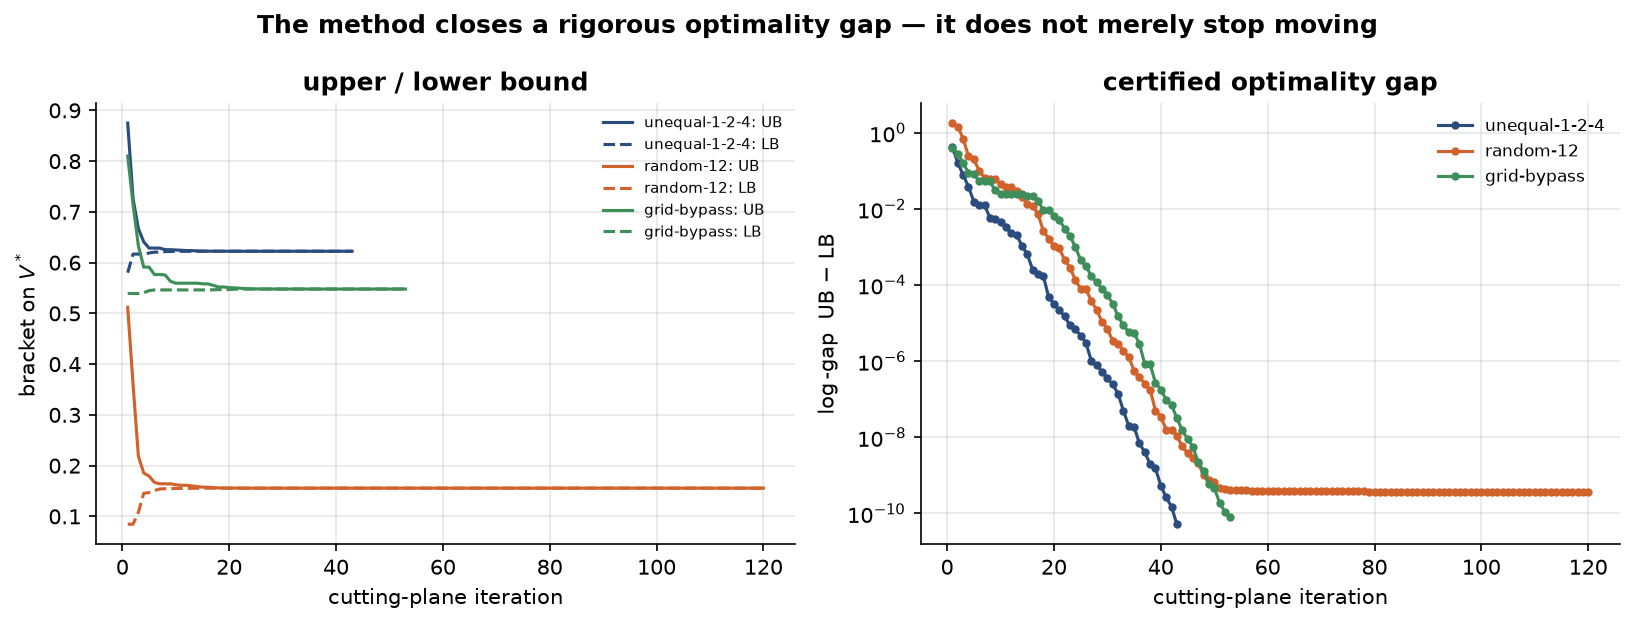
\includegraphics[width=0.95\columnwidth]{figs/E6_convergence.png}
\caption{Left: upper and lower bounds on $V^{\star}$ converge. Right: the gap
falls by roughly ten orders of magnitude before flattening at the limits of
floating-point precision. Generated by \texttt{experiments.py}, experiment
E6.}
\label{fig:convergence}
\end{figure}

\subsection{Contest Intensity}

Varying $m$ over $\{0.25,0.5,0.75,1,1.5,2,3\}$ separates two regimes. On a
single chain with $\XA=\XB$ the value is flat at $0.0625$ for every $m$,
since equal budgets force $p_i=\tfrac12$ at any intensity. On grid-4x4 the
value rises from $0.1177$ at $m=0.25$ to $0.9399$ at $m=3$. Where the
defender must spread over parallel routes while the evader concentrates on
one, economies of scale favour the evader. The $m>1$ half of this sweep is
exploratory and is reported as not certified.

\subsection{A Valid Bracket for $m>1$}
\label{sec:results-mgt1}

The hull relaxation of Section~\ref{sec:convexity} yields a two-sided bracket
where no certificate is available. On the diamond graph at $m=2$ it gives
$V^{\star}\in[0.667,0.800]$, the endpoints being $2/3$ and $4/5$. The
relaxation is valid on all 15 instances tested but weak: the slack does not
shrink as the solver converges, and it widens with $m$, from $10.8\%$ at
$m=1.5$ on the diamond to $12400\%$ at $m=3$ on a three-node chain. It
brackets the value; it never certifies that an allocation is optimal.

%==============================================================================
\section{DISCUSSION}
\label{sec:discussion}

The practical message is that plausible defensive intuitions are unreliable.
Spreading a budget evenly and protecting the choke point are both
defensible-sounding rules, and both can be far from optimal. The reason is
the same in each case: neither accounts for how route length interacts with
the contest at each node. A long route already punishes the evader through
repeated multiplication, by \eqref{eq:symmetric}, so a short route needs more
defence per node. Rules that allocate by node count or by how many routes
pass through a node systematically under-defend short routes.

The value of a certified method rather than a heuristic one is that it
reports how far from optimal an alternative allocation is.
Table~\ref{tab:e3} and Table~\ref{tab:e9} would not be meaningful without
first solving for the true optimum, and the comparison in
Section~\ref{sec:results-h2h} shows that this remains the operative
difference even against methods that land within a few per cent.

\paragraph{Limitations.}
Contest intensity above $1$ is not certified: convexity provably fails
(Proposition~\ref{prop:m-gt-1}), and the hull relaxation gives a valid but
weak bracket rather than a certificate. Whether any solution concept can be
characterised in that regime is open. The game is sequential; a simultaneous
version would generally require mixed strategies over routes
\citep{nguyen2023}. We show empirically that the method converges but prove
no rate; Kelley's method can converge slowly and its complexity depends on
problem geometry \citep{nesterov2018}, and
Proposition~\ref{prop:partial-strict} is a natural starting point for a rate
we have not attempted. The payoff is a product of per-node survival
probabilities, which assumes detection events at different checkpoints are
independent; real checkpoints often share information, which would break the
separability the shortest-path reduction depends on. Contests are modelled on
nodes, with edge contests obtained by a line-graph relabelling. The route
oracle is certified but not guaranteed fast, and in the worst case can
degrade to examining every route. The comparison in
Section~\ref{sec:results-h2h} uses adaptations of the two nearest methods
rather than the published implementations, since neither applies verbatim to
this model. Finally, Proposition~\ref{prop:uniqueness} and
Theorem~\ref{thm:convexity} are proofs, and automated testing can refute but
never confirm a proof; both warrant independent checking, particularly given
the retracted argument noted in the remark of Section~\ref{sec:convexity}.
The literature search behind Section~\ref{sec:related} is a keyword search,
not a systematic review.

%==============================================================================
\section{CONCLUSIONS}
\label{sec:conclusion}

A defender with a fixed budget, facing an evader who chooses both a route and
an effort at each checkpoint on it, faces a problem that looks intractable:
an exponential number of routes and an objective that is neither convex nor
concave as written. In logarithmic coordinates the problem is convex whenever
the contest intensity does not exceed $1$, which makes a certified global
optimum reachable, and we give an explicit graph on which convexity fails
above that threshold. The optimal allocation is unique when the game is
non-degenerate, proved by a covering argument rather than by strict
convexity, which fails here.

Algorithmically, a Lagrangian relaxation that is additive across nodes turns
the route search into a single shortest-path computation together with a rule
that proves when the search may stop, and the outer allocation problem yields
to cutting planes with a stabilised master. On layered graphs with up to
$1.68\times10^{7}$ routes the oracle examines two routes per best response
and all 13 outer certificates close.

Three directions follow from the limitations rather than from generic
extension. The $m>1$ regime currently admits only the hull bracket of
Section~\ref{sec:results-mgt1}, and a genuinely global method there would
need either a tighter convexification or a mixed-strategy characterisation.
The convergence rate of the stabilised master is unproven, and
Proposition~\ref{prop:partial-strict} is the natural handle on it. Relaxing
independence across checkpoints would break the additivity that
\eqref{eq:sp-bound} depends on, and it is not obvious what replaces the
shortest-path oracle if it goes.

%==============================================================================
\section*{ACKNOWLEDGEMENTS}

% TODO(author): add funding and institutional acknowledgements here.

AI tools were used solely for language editing, grammar checking, and
improving the clarity of the manuscript. This assistance was provided by
Claude (Anthropic) and applied to the manuscript text throughout rather than
to any particular section. All mathematical analysis, research
contributions, proofs, experimental work, interpretation of results, and
scientific conclusions are the responsibility of the authors.

%==============================================================================
\begin{thebibliography}{99}
\setlength{\itemsep}{0pt}

\bibitem[Bloch et al.(2023)]{bloch2023}
F.~Bloch, K.~Chatterjee, and B.~Dutta.
\newblock Attack and interception in networks.
\newblock \emph{Theoretical Economics}, 18(4):1533--1571, 2023.

\bibitem[Bozbay and Vesperoni(2018)]{bozbay2018}
I.~Bozbay and A.~Vesperoni.
\newblock A contest success function for networks.
\newblock \emph{Journal of Economic Behavior and Organization},
  150:404--422, 2018.

\bibitem[Danskin(1967)]{danskin1967}
J.~M. Danskin.
\newblock \emph{The Theory of Max-Min and its Application to Weapons
  Allocation Problems}.
\newblock Springer, 1967.

\bibitem[Hausken(2008)]{hausken2008}
K.~Hausken.
\newblock Strategic defense and attack for series and parallel reliability
  systems.
\newblock \emph{European Journal of Operational Research}, 186(2):856--881,
  2008.

\bibitem[Iliaev et al.(2023)]{iliaev2023}
D.~Iliaev, S.~Oren, and E.~Segev.
\newblock A Tullock-contest-based approach for cyber security investments.
\newblock \emph{Annals of Operations Research}, 320:61--84, 2023.

\bibitem[Israeli and Wood(2002)]{israeli2002}
E.~Israeli and R.~K. Wood.
\newblock Shortest-path network interdiction.
\newblock \emph{Networks}, 40(2):97--111, 2002.

\bibitem[Kelley(1960)]{kelley1960}
J.~E. Kelley.
\newblock The cutting-plane method for solving convex programs.
\newblock \emph{Journal of the SIAM}, 8(4):703--712, 1960.

\bibitem[Kovenock and Roberson(2018)]{kovenock2018}
D.~Kovenock and B.~Roberson.
\newblock The optimal defense of networks of targets.
\newblock \emph{Economic Inquiry}, 56(4):2195--2211, 2018.

\bibitem[Marsten et al.(1975)]{marsten1975}
R.~E. Marsten, W.~W. Hogan, and J.~W. Blankenship.
\newblock The boxstep method for large-scale optimization.
\newblock \emph{Operations Research}, 23(3):389--405, 1975.

\bibitem[Nesterov(2018)]{nesterov2018}
Y.~Nesterov.
\newblock \emph{Lectures on Convex Optimization}.
\newblock Springer, 2nd edition, 2018.

\bibitem[Nguyen et al.(2023)]{nguyen2023}
D.~H. Nguyen, J.~Song, and J.~C. Smith.
\newblock Network interdiction with asymmetric information and evasion.
\newblock \emph{Networks}, 81(4):447--468, 2023.

\bibitem[Oruganti et al.(2023)]{oruganti2023}
P.~S. Oruganti, P.~Naghizadeh, and Q.~Ahmed.
\newblock The impact of network design interventions on the security of
  interdependent systems.
\newblock arXiv:2302.05411, 2023.

\bibitem[Ramirez-Marquez et al.(2011)]{ramirez2011}
J.~E. Ramirez-Marquez, C.~M. Rocco, and G.~Levitin.
\newblock Optimal network protection against diverse interdictor strategies.
\newblock \emph{Reliability Engineering and System Safety}, 96(3):374--382,
  2011.

\bibitem[Skaperdas(1996)]{skaperdas1996}
S.~Skaperdas.
\newblock Contest success functions.
\newblock \emph{Economic Theory}, 7(2):283--290, 1996.

\bibitem[Smith and Song(2020)]{smith2020}
J.~C. Smith and Y.~Song.
\newblock A survey of network interdiction models and algorithms.
\newblock \emph{European Journal of Operational Research}, 283(3):797--811,
  2020.

\bibitem[Tullock(1980)]{tullock1980}
G.~Tullock.
\newblock Efficient rent seeking.
\newblock In \emph{Toward a Theory of the Rent-Seeking Society}, pages
  97--112. Texas A\&M University Press, 1980.

\bibitem[Washburn and Wood(1995)]{washburn1995}
A.~Washburn and K.~Wood.
\newblock Two-person zero-sum games for network interdiction.
\newblock \emph{Operations Research}, 43(2):243--251, 1995.

\bibitem[Yen(1971)]{yen1971}
J.~Y. Yen.
\newblock Finding the $k$ shortest loopless paths in a network.
\newblock \emph{Management Science}, 17(11):712--716, 1971.

\end{thebibliography}

\end{document}
